\documentclass[11pt,a4paper,oneside]{scrreprt}
\usepackage{sastyle}
\usepackage{longtable}
\usepackage{wrapfig}
\setcounter{secnumdepth}{3}


% Title Page
\title{metriculator - CDT metric plug-in}
\author{Ueli Kunz, Julius Weder}


\begin{document}
\pagenumbering{alph}
\begin{titlepage}
\topmargin 0in
% \maketitle
\thispagestyle{empty}
\begin{center}


\begin{figure}[hp]
  \begin{minipage}[t]{0.5\textwidth}
	\vspace{0pt}
    
\includegraphics[scale=0.25]{figures/HSR.jpg}
  \end{minipage}
  \hfill
  \begin{minipage}[t]{0.5\textwidth}
	\vspace{-2.5pt}
    
\includegraphics[scale=0.35]{figures/IFS.jpg}
  \end{minipage}
\end{figure}


\vspace{1,5cm}
{\Large \bfseries HSR -- University of Applied Sciences Rapperswil\\}
\vspace{0,25cm}
{\Large \bfseries Institute for Software\\}
\vspace{1cm}
{\Large \bfseries Semester Thesis\\}
\vspace{2cm}
\sffamily
{\Huge \bfseries metriculator}\\
\vspace{0.5cm}
{\Huge \bfseries CDT metric Plug-in}\\
\vspace{1cm}
Ueli Kunz, \url{ukunz@hsr.ch}\\
Julius Weder, \url{jweder@hsr.ch}
\\\vspace{1,0cm}
\begin{scriptsize}\url{http://sinv-56013.edu.hsr.ch}\\\end{scriptsize}
\vspace{1.5cm}
Supervised by Prof. Peter Sommerlad\\
\vspace{0,3cm}
\today
\end{center}
\end{titlepage}


\clearpage\pagenumbering{roman}

\newpage
\thispagestyle{empty}
\mbox{}
\setcounter{page}{0}
\newpage

\chapter*{Abstract}
This thesis aims at statically analysing software written in C++ using known software metrics. Software metrics are used to obtain objective, reproducible and quantifiable measurements of source code. This measurements may support various tasks such as performance optimization, quality assurance testing or software debugging \cite{wiki_softwaremetric}.\\
Metriculator is programmed in Java and integrates in Eclipse as plug-in that depends on the Codan \cite{codan} framework which is part of the C/C++ Development Tooling platform (CDT, \cite{CDT}). Codan is a code analysis framework that offers a mechanism to add new code analysis features. Each metric in metriculator is implemented as an extension to Codan. First and foremost it is about extracting meaningful information out of C++ source code using different software metrics.
\\\\
After analysing the code, the results are shown in the metriculator view, which provides different representations of the same underlying data. Additionally the metriculator view helps finding problems and moving to their problematic source code sections. Optionally the detected problems will be displayed as markers with detailed problem information within the source code editors. Each metric can be activated or deactivated and as well have variable threshold values that suite the needs of the specific domain.
\\\\
There are five metrics already implemented and it is possible to extend metriculator with additional metrics without touching the existing source code.
Implemented metrics:
\begin{itemize}
\item Number of Logical Source Lines of Code (LSLOC)
\item Cyclomatic Complexity (McCabe)
\item Number of Parameters per Function
\item Number of Members per Type
\item Efferent Coupling per Type
\end{itemize}

\newpage
\thispagestyle{empty}
\mbox{}
\newpage

\chapter*{Management Summary}
This chapter summarises the goals and outcomes of this thesis. And gives a preview on what might be possible in the future.

\section*{Initial Situation}
Various aspects of source code can be expressed in numbers. Such an aspect is called a software metric. For instance, a well known software metric measures the number of lines of code. Software metrics allow users to view the analysed source code from different perspectives. They may give a high level overview of the size and quality of the analysed source code. But they can also help developers to identify problematic source code sections.

Static analysis tools investigate source code without running the application itself. Many static analysis tools exist for various programming languages \cite{metrictools}. But at the time of this project, there was no metric tool available that integrates into the Eclipse C/C++ Development Tooling platform (CDT, \cite{CDT}). Our goal was to create the first static source code analysis tool for CDT.

\section*{Procedure and Technologies}
metriculator is a plug-in for CDT that itself is a plug-in of the Eclipse framework. CDT is a well known platform to develop C/C++ software. Beside CDT, metriculator uses a framework called Codan \cite{codan} to analyse C++ source code. Codan is extensible so that third party tools such as metriculator can hook in and add their own code analysis features.\\
Metriculator analyses a user defined set of files. The analysis results are applied to functions, classes, namespaces, files, folders and projects. The analysis results are viewable using different views that all rely on the same underlying data.

\section*{Results}
Metriculator supports the following five software metrics, each of which is described in detail in section \ref{metric-spec}.

\begin{description}
\item[Logical Source Lines of Code] numbers the size of the software by counting the lines of code. See \ref{lsloc} for detailed description.
\item[Cyclomatic Complexity] also called McCabe, is an indicator for the complexity of the software. For instance many \textit{if} statements increase the complexity and lead to unreadable and hard to maintain code. See \ref{mccabe} for detailed description.
\item[Number of Parameters per Function] measures the number of parameters of a function. See \ref{nbparams} for detailed description.
\item[Number of Members per Type] measures the number of members of a class, struct or union. See \ref{nbmembers} for detailed description.
\item[Efferent Coupling] counts the number of foreign types a certain type depends on. For instance, many dependencies indicate highly coupled software. See \ref{effcoupling} for detailed description.
\end{description}

Compared to the specified objectives at the start of the project there are two metrics missing. The Number of Nested Levels
and the Number of Template Parameters metric were not implemented. This is because we decided to implement the Efferent Coupling metric in advance and because of the unforeseen performance issues that must have been resolved prior to additional feature implementations. See \ref{performance-tuning} for more details.
\\\\
Metriculator is available as Eclipse plug-in and can be installed from within Eclipse using the install wizard. After installation, users can run the Codan code analysis. As part of this analysis, metriculator will run as well. The gathered metric data can be investigated using different views provided by metriculator.

\subsection*{Illustrated Example}
In this section we will explain the results, shown in the metriculator views, after analysing a sample project.\\
\begin{description}
\item[Default View] Figure \ref{fig:metriculator_hybrid} shows a screenshot of the default metriculator view after the static code analysis ran. The default view shows all analysed files and folders in a tree view. Files can further be expanded to explore the source code they contain. The values of each metric are displayed in a separate sortable column. Each row represents one analysed scope.
\item[Warnings] As visible in Figure~\ref{fig:metriculator_hybrid} \textit{func3} has seven parameters. Because seven is above the threshold set in the metric preferences the cell is highlighted.
\item[Filter View] The filter view in Figure~\ref{fig:metriculator_filter} shows all functions. Other filters can be applied to see a list of only files, types or namespaces. Thanks to the filter view, users are able to quickly identify large files for instance.
\item[Data Visualisation] Metric values can also be visualised in a tag cloud, as illustrated in Figure~\ref{fig:tagcloud} using the LSLOC metric values. The bigger the font size of the function name, the higher its metric value is.
\end{description}

\begin{figure}[th]
\begin{center}
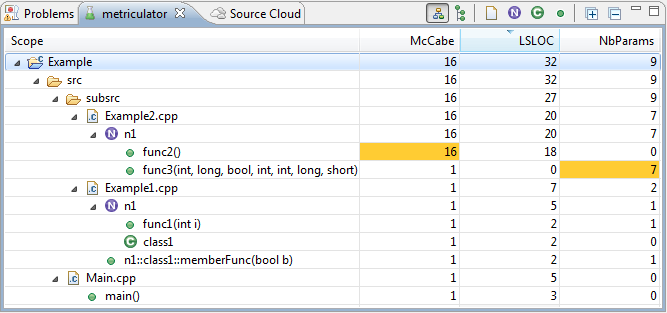
\includegraphics[width=\textwidth]{figures/hybrid_view.png}
\end{center}
\caption{Screenshot of the metriculator hybrid view.}
\label{fig:metriculator_hybrid}
\end{figure}

\begin{figure}[th]
\begin{center}
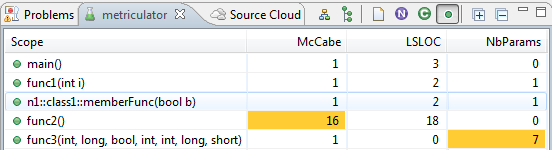
\includegraphics[]{figures/filtered_functions_view.png}
\end{center}
\caption{Screenshot of the metriculator filter view listing all functions.}
\label{fig:metriculator_filter}
\end{figure}

\begin{figure}[th]
\begin{center}
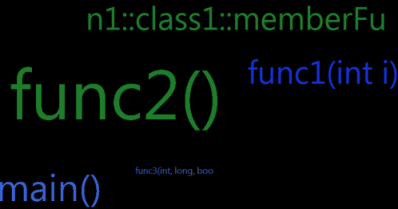
\includegraphics{figures/tag_cloud_lsloc.png} 
\end{center} 
\caption{Generated tag cloud that visualises the LSLOC value of all functions.}
\label{fig:tagcloud}
\end{figure}

\section*{Future Work}
There are many interesting not yet implemented metrics that would increase the value of metriculator, see chapter \ref{advobjectives} for an incomplete list.\\
Performance can further be improved to allow analysing source code with over about 300'000 physical lines of source code. Fixing that issue would make metriculator even more attractive to analyse large projects. Other unresolved issues are listed in chapter~\ref{knownissues}.\\
A reasonable application of metriculator in the future is to serve as refactoring assistant. Based on a reported problem, metriculator could suggest a refactoring or quick fix that solves that problem.

\cleardoublepage
\newpage
\thispagestyle{empty}
\mbox{}
\newpage

\setcounter{tocdepth}{2}
\tableofcontents

\vspace{3cm}

\begin{center}
\textit{Experience is a hard teacher because she gives the test first, the lesson after ward.}
\\
\begin{flushright}
Vernon Law
\end{flushright}
\end{center}

\pagebreak
\clearpage\pagenumbering{arabic}
\chapter{Introduction}\label{Introduction}
The investigation of source code has ever since been an important task in software development \cite{historystaticanalysis}. Static source code analysis is one type of source code investigation with the objective to get a picture of the written code itself. One output of static source code analysis are source code metrics. Many types of metrics exist since source code can be inspected under different aspects. For instance the lines of code metric gives an impression about the size of the code.\\
Many metric analysis tools for almost any programming language already exist. But at the time of this semester thesis there was no official C++ metric tool available that integrates well in to the Eclipse CDT (C/C++ Development Tooling) platform \cite{CDT}.

\section{Motivation}
We intend to improve the quality of the Eclipse CDT platform as it will help other developers to create better software. Code metrics provide a big picture of the quality of the source code. There are plenty of well known and also standardised code measurement techniques around and implemented for other tools and languages. We give our best to implement these techniques and standards for the CDT platform.

\section{Objectives}

\begin{description}
\item[Project organization] Fixed one-week iterations are used. Redmine \cite{redminesetup} is used for planning, time tracking, issue tracking and as information radiator for the supervisor. A project documentation is written. Organization and results are reviewed weekly together with the supervisor.

\item[Integration and Automation] Sitting in front of a fresh Eclipse CDT installation a first semester student can install our metric plug-in using an update site as long as metriculator is not integrated into the main CDT plug-in. An update site is created to allow the installation of metriculator using the Eclipse install wizard.

\item[Quality] The plug-in code is covered with automated test cases. Automated UI tests are not mandatory.

\item[Delivered Assets] At the end, the project will be handed to the supervisor with two CDs and two paper versions of the documentation. The CDs contain: this project report, a video demonstrating the usage of metriculator, the source code and the deployable plug-in.

\item[Implemented metrics] The metrics listed below are going to implemented with highest priority.
\begin{itemize}
\item Number of Members per Class
\item Lines of Code per File
\item Lines of Code per Class
\item Lines of Code per Function
\item Cyclomatic Complexity (McCabe) per Function
\item Number of Nested Levels
\item Number of Template Parameters
\item Number of Parameters per Function
\end{itemize}

\end{description}

\subsection{Advanced Objectives}\label{advobjectives}
If the basic objectives get finished before the end of the project, we may start implementing the following metrics:
\begin{itemize}
\item Number of References of Type (class, struct, union)
\item E/Afferent Coupling
\item Feature Envy
\item Lack Of Cohesion per Function
\item Number of Overloads
\item Depth of Inheritance Tree
\item Instability
\item Abstractness
\item Normalized Distance from Main Sequence
\item Number of Locals in Scope
\item Number of Lines of Code vs Lines of Comment (Density of Comments)
\end{itemize}

\subsubsection{Tag Cloud Integration}
Tag clouds are an excellent way to visualise weighted data. The Sourcecloud plug-in for Eclipse \cite{sourcecloud_git} generates a tag cloud of all words in source code files. The view of that plug-in could be integrated in our plug-in to visualise weighted data of one metric. For instance, the LSLOC values of all functions. A higher LSLOC value results in a bigger font size of the function name.

\section{Project Duration}
The semester thesis starts on September 19th and has to be finished until December 23rd, 2011.

\chapter{Requirements}\label{requirements}
This chapter describes the functional and non functional requirements of the metriculator plug-in.

\section{metriculator view}\label{metriculator-view}
This view is able to show the data of all metrics for different scopes. It visualises the underlying data in three different views.

\begin{description}
\item[hybrid view] is the default view and shows the projects and its content as a mix of physical and logical representation in a tree. This is the default view and shows a tree view representing the file system structure of the investigated files and folders, where the files further contain the logical tree structure that is a simplified form of the abstract syntax tree (AST) of the file contents. The following node types are displayed:

\begin{itemize}
\item project
\item folder
\item file
\item namespace
\item type (class, struct, union)
\item function
\end{itemize}
\begin{figure}[hp]
 \centering
	 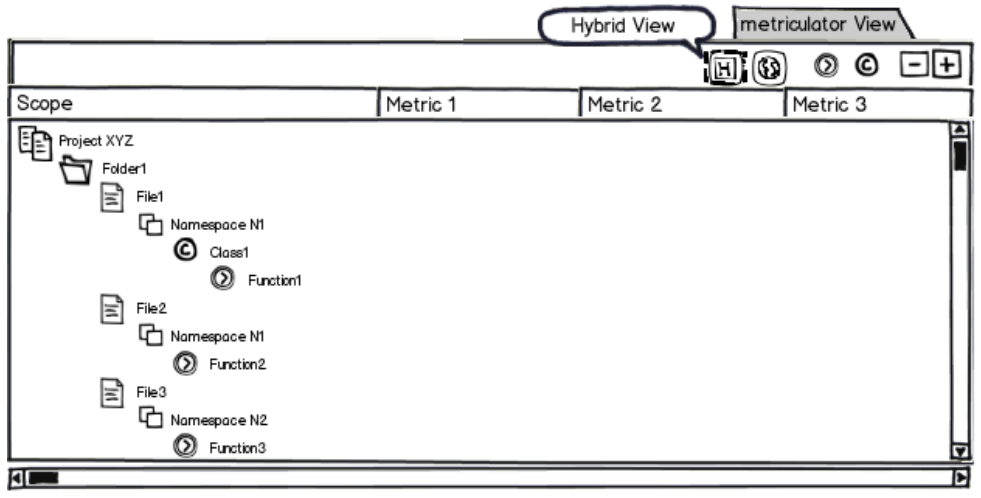
\includegraphics[scale=0.5]{figures/HybridView.png}
 \caption{Hybrid view}
   \label{fig:hybrid_view}
\end{figure}

\item[logical view] shows the logical representation of the source code in one tree. This view merges the logical trees of all files and thus does not show any file system information. The following node types are displayed:
\begin{itemize}
\item namespace
\item type (class, struct, union)
\item function
\end{itemize}

\begin{figure}[hp]
 \centering
 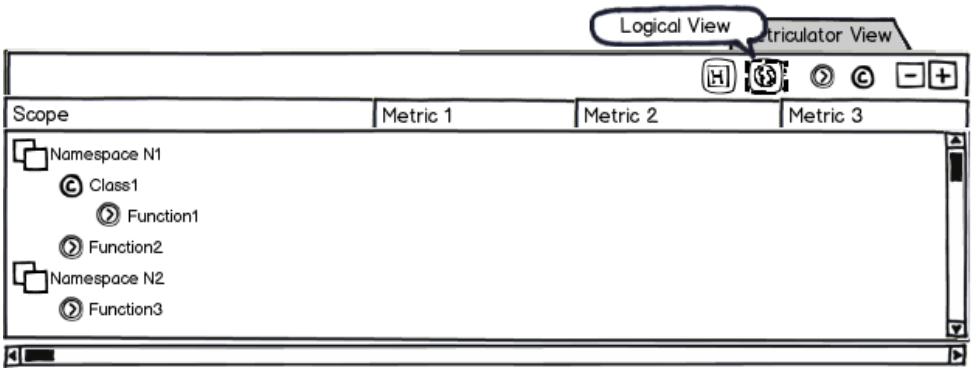
\includegraphics[scale=0.5]{figures/LogicalView.png}
 \caption{Logical view}
    \label{fig:logical_view}
\end{figure}

\item[filter view] shows a flat representation of all hybrid tree nodes. The node list can be filtered by the different types of nodes. Following filters exist:
\begin{itemize}
\item file
\item namespace
\item type (class / struct / union)
\item function
\end{itemize}
\begin{figure}[hp]
 \centering
 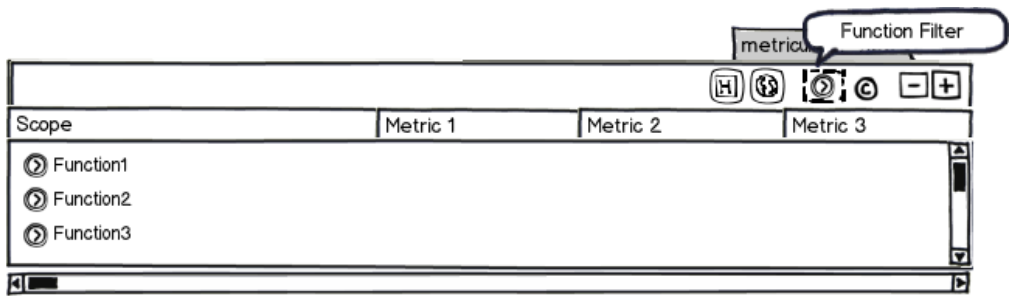
\includegraphics[scale=0.5]{figures/FilteredView.png}
 \caption{Filter view}
    \label{fig:filtered_view}
\end{figure}

\item[tag cloud view] is another nice way of visualising metric values by generating a tag cloud that allows fast visual detection of potentially problematic items such as large functions or high coupled classes (Figure \ref{fig:tag_cloud_mockup}).
\begin{figure}[th]
 \centering
 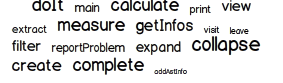
\includegraphics[scale=0.5]{figures/tag_cloud_mockup.png}
 \caption{Tag cloud view}
    \label{fig:tag_cloud_mockup}
\end{figure}

\end{description}
In all views the columns can be sorted ascending or descending, by scope name or metric value. The nodes in the tree structure can be expanded and collapsed (fully or partially).

\section{Use Cases (Brief Format)}
The following use cases apply to all implemented metrics.
\subsection{Starting the Metrics Analysis}
A user chooses some C++ projects he wants to analyse and runs the Codan command in Eclipse. All calculated metrics will be displayed in the metriculator view.
\subsection{Change Metric Configuration}
A user can change the configuration of the Lines of Code metric by specifying an individual range of acceptable thresholds. The view marks the values outside of the thresholds.
\subsection{Visualise Metric as tag cloud}
The user chooses a metric in the metriculator view. Metriculator generates a tag cloud which visualises the values of the selected metric.
\subsection{Analyse Metric Results}
The user has run the analysis and the metriculator view is shown. He can now switch between the different views, sort columns, or generate a tag cloud.

\chapter{Metric Specification}\label{metric-spec}
This chapter specifies the details of the implemented metrics. Most metric implementations follow standards (specified in sub chapters) with some extensions where required by C++. Each metric specification describes what the metric means, which scopes it applies to and how it is measured.

\section{Logical Source Lines of Code (LSLOC)}\label{lsloc}
Source Lines Of Code (SLOC, or Lines Of Code) \cite{lsloc_def} is a unit used to measure the size of software programs. There exist different types of Lines Of Code (LOC) metric definitions. Some count the number of statements, others count the physical lines of source code (with or without comments) or even the number of byte code instructions. We decided to use the term LSLOC (Logical Source Lines of Code) because the University of Southern Carolina defines a standard for LSLOC counting rules for C++ \cite{lsloc_def}.\\
As long as not otherwise noted metriculator respects the rules of this standard. Because this standard does not define rules for some of the new concepts of the C++11 \cite{cpp_11_std} standard, especially lambdas, we defined new rules where required.

\subsection{Lambda Expressions}
\begin{lstlisting}[style=C++0x, caption=Lambda expression code snippet with LSLOC of 4, label=lsloc_lambda]
int z, x;
auto square = 						
		[z, x]				// 1 - one lambda-capture, two captures
			()
			  { 			// 1 - function body
				return z*z;	// 1 - statement
			  }
			  ;				// 1 - assignment statement
\end{lstlisting}

As illustrated in listing \ref{lsloc_lambda}, the following rules apply to lambda expressions:
\begin{enumerate}
\item A lambda-capture counts one, regardless of the number of captures it contains.
\item Anonymous function declaration counts one (as any other function declaration does).
\item Statements in the lambda body count as usual.
\item The assignment of the lambda expression to \textit{square} counts one (as any other assignment).
\item Direct calls of lambda expressions (no assignment) count one.
\end{enumerate}

In contrast to other function declarations, lambdas may have a lambda-capture that increases the LSLOC value by one.

\subsection{Enum}
\begin{lstlisting}[style=C++0x, caption=Enum code snippet with LSLOC of 1, label=lsloc_enum]
enum x{
	val1,
	val2
} // 1 - type definition
\end{lstlisting}

As illustrated in listing \ref{lsloc_enum}, the following rules apply to enums:
\begin{enumerate}
\item An enum declaration counts one.
\item Enum values do not count.
\end{enumerate}

\section{McCabe (Cyclomatic Complexity, CC)}\label{mccabe}
The McCabe metric, also known as Cyclomatic Complexity \cite{mccabe_def}, is a software metric for measuring the complexity of parts of a software. This metric indicates whether a piece of code is still comprehensible to humans. Simply expressed it is the number of binary branches plus one.

Our implementation is based on a paper published by Verifysoft Technology GmbH \cite{mccabe_def}.
\subsection{Example}
\begin{lstlisting}[style=C++0x, caption=Code snippet example McCabe, label=mccabe_example]
namespace n1 { // 1 + 2 + 1 - 2 = initial + func1 + func2 - #children

	int func1(int i){ // 1 + 1
		if(i < 0){ // 1
			return 0;
		}
		return 0;
	}

	int func2(int){ // 1
		return 1;
	}
}
\end{lstlisting}

Every node has an initial Cyclomatic Complexity of 1. In listing \ref{mccabe_example} the function \textit{func1} has due to the \textit{if} statement a Cyclomatic Complexity of 2. The parent node of the two functions has therefore a Cyclomatic Complexity of 2. To build the node value of a parent node, all children node values are summed up. Afterwards the sum of the parent is decremented by the number of children.

\section{Number of Parameters per Function}\label{nbparams}
The Number of Parameters per Function metric is a software metric, that counts the amount of parameters in a function or member function. All parameters are counted. This metric is an indicator whether a function is painful to call or maybe degrade performance.
\subsection{Exceptions}
\begin{enumerate}
\item If a function definition has a forward declaration, the parameters of the forward declaration are not counted. Following Listing~\ref{nbParamsDecl_example} illustrates an example:
\begin{lstlisting}[style=C++0x, caption=Code snippet for Number of Parameters per Function - function declarations and definitions, label=nbParamsDecl_example]
int doIt(int, bool);	// does not count because of the definition below
int doAnother(int, bool);	// counts 2 parameters

int doIt(int i, bool b){	// counts 2 parameters
	return b ? i : 0;
}
\end{lstlisting}

\item If a member function declaration has an associated definition, the parameters are not counted in the logical view but they are counted in the hybrid view, expect they are in the same file, then the hybrid view also does not count the function declaration. Following Listing~\ref{nbParamsMemberDecl_example} illustrates an example:
\begin{lstlisting}[style=C++0x, caption=Code snippet for Number of Parameters per Function - member function declarations and definitions, label=nbParamsMemberDecl_example]
class Example{
public:
	void doIt(int, bool);	// does not count because of the definition below
	void doAnother(int, bool);	//counts 2 parameters
};

void Example::doIt(int i, bool b){	//counts 2 parameters
	// do something
}
\end{lstlisting}
\end{enumerate}

\section{Number of Members per Type}\label{nbmembers}
The Number of Members per Type metric is a software metric that counts the members of a type. A types can be a \textit{class}, \textit{struct} or \textit{union}. \\
Our implementation is based on the official C++11 Standard \cite{cpp_11_std} especially on the chapter Class Members. As long as not otherwise noted, metriculator respects the rules in this standard.
\subsection{Explanation of Member Types}
There are three different kinds of members:
\begin{enumerate}
\item data members
\item member functions
\item nested types
\begin{enumerate}
\item class
\item struct
\item union
\item enum
\item typedef declaration
\end{enumerate}
\end{enumerate}

Members are counted whatever visibility they have. Nested types can be anonymous. Members are not counted if they are friend classes or member functions.\\
Listing~\ref{nbMembers_example} illustrates an example:
\begin{lstlisting}[style=C++0x, caption=Code snippet for Number of  Members per Type, label=nbMembers_example] 
class Example{
	int i;	// counts 1
public:
	class NestedExample1;	// counts 1
	struct NestedExample2{	// counts 2 (itself as nested type and its member)
		int i;	// counts 1
	};
	enum{a,b,c};	// counts 1
	typedef int myInt;	// counts 1
	void doIt();	// counts 1
	friend class MyFried;	// does not count
	friend void doAnother();	// does not count
};
void doNothing();	// does not count
\end{lstlisting}

\section{Efferent Coupling}\label{effcoupling}
Efferent Coupling is a metric that numbers on how many distinct foreign units the unit of interest relies on. Metriculator implements Efferent Coupling on type level. That means that the more foreign types a type depends on, the higher its efferent coupling value is. A dependency exists if a type is directly referenced.\\
Following Listing~\ref{efferentCoupling_example} illustrates an example:
\begin{lstlisting}[style=C++0x, caption=Code snippet for Efferent Coupling, label=efferentCoupling_example] 
class Example2;
class Example3;

class Example1 {
public:
	void doSomething(Example2 *e2) {};	// counts 1 for type Example1
	Example3 ex3();		// counts 1 to type Example 1
};

class Example2 {
public:
	void doSomething(Example1 *e1) {};	// counts 1 for type Example2
};

class Example3{
};
\end{lstlisting}

\chapter{Implementation}
This chapter describes the main classes and concepts of the metriculator plug-in. First we give an overview of the package level architecture. Then we dive into the details of the model package by commenting static and dynamic aspects. At the end some performance related actions as well as known issues will be presented in detail.

\section{Plug-in Architecture}
As visible in Figure~\ref{fig:cdt_codan_components_impl} metriculator is based on the Codan framework. Codan uses checkers to analyse source code. Each checker is specialised in one problem, for instance unreachable code. Through extension points Codan allows third party tools to register other checkers. Metriculator defines one checker per metric. As soon as a user invokes the Codan command on the UI, Codan automatically calls all registered checkers.\\
The metriculator component in Figure~\ref{fig:cdt_codan_components_impl} can further be divided into the packages shown in Figure~\ref{fig:metriculator_packages}.
\begin{figure}[th]
 \centering
 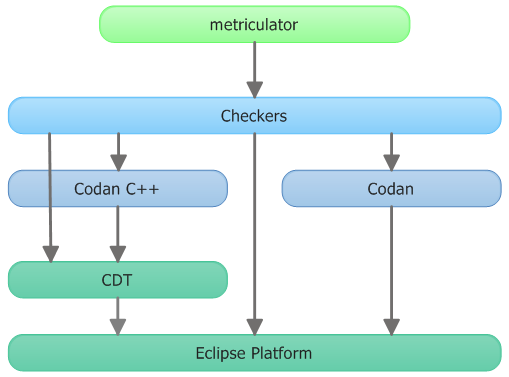
\includegraphics[scale=0.6]{figures/cdt_codan_components.png}
  \caption{Architectural representation of the components metriculator relies on.}
  \label{fig:cdt_codan_components_impl}
 \end{figure}

\begin{figure}[th]
\begin{center}
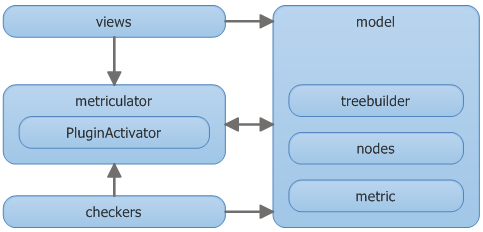
\includegraphics{figures/model_metriculator_packages.png}
\end{center}
\caption{Package diagram with packages inside the metriculator plug-in.}
\label{fig:metriculator_packages}
\end{figure}

The metriculator package is the core of this plug-in. Thanks to the \textit{PluginActivator} we know when the Codan command is started and finished. This allows us to initialise the model each time before the checkers start working. After the work is done the \textit{PluginActivator} notifies the views to update their data via observer. As the checkers run they build a tree model that represents the analysed files and their content.\\
The bidirectional dependency between the model and the metriculator component exists because some model classes use a singleton inside of the metriculator component. Singletons are used due to constraints of the Eclipse framework.

\subsection{Plug-in Activator}
The plug-in activator activates the plug-in when it is about to run.
Every Eclipse plug-in inherits from the \textit{AbstractUIPlugin} of Eclipse. The \textit{MetriculatorPluginActivator} holds the singleton instance of this plug-in. The constructor of the \textit{MetriculatorPluginActivator} registers itself at a job listener which notifies metriculator when Codan starts the code analysis and when Codan has done its job.\\
Before the metriculator plug-in starts its job, it has to reset all model data. The job listeners also reset the caches of the metric values, clear the views and models to dereference all old objects from a previous execution of metriculator. See \ref{performance-tuning} for further information.\\
All metric checkers has to register themselves at the \textit{MetriculatorPluginActivater}.
After Codan has finished its job, the \textit{MetriculatorPluginActivator} invokes the aggregation of all values of the activated metrics and shows the metriculator view. \textit{MetriculatorPluginActivator} has a \textit{JobObservable} that implements the \textit{Observable} and is responsible for notifying his observers if the plug-in is about to run or if its job is done. Observers of the \textit{JobObservable} are the metriculator view and all metric checkers.

\begin{figure}[th]
\begin{center}
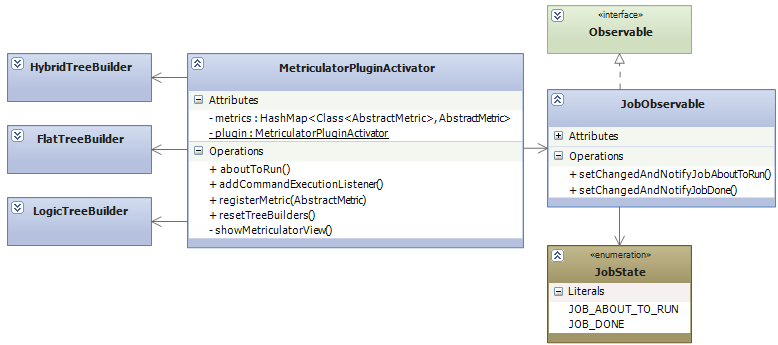
\includegraphics[scale=0.8]{figures/pluginactivator.png}
\end{center}
\caption{Class diagram with classes related to \textit{MetriculatorPluginActivator}}
\label{fig:plugin_activator}
\end{figure}

\section{Tree Structure}
This sections describes the composite tree structure that is build by the \textit{AbstractMetricChecker} instances during the processing described in Chapter \ref{processing}. This tree structure holds all the data shown in the metriculator view.

\subsection{TreeBuilder}\label{treebuilder}
As illustrated in Figure~\ref{fig:model_treebuilder} metriculator uses three different tree models which correspond to the three different views. The hybrid tree model is used in the hybrid view, the logical tree model is used in the logical view and the flat tree model is used in the filter view.\\
The \textit{TreeBuilder} class is an abstract factory that is used by the checkers to create tree models. \textit{AbstractMetricChecker} uses a \textit{HybridTreeBuilder} to add new nodes to the tree structure. During the processing only the hybrid tree model is build because the hybrid tree model holds all the information that other tree models require. Flat trees and logical trees are build on demand using the data of the hybrid tree model. For instance, when a user switches from the hybrid view to the logical or filter view. \textit{FlatTreeBuilder} and \textit{LogicalTreeBuilder} use a \textit{PreOrderTreeVisitor} to visit all nodes in the hybrid tree model and transform it to the new respective tree model.\\
The class factory method \textit{createTreeFromPath(IPath)} is used by the \textit{HybridTreeBuilder} to create a tree structure that represents a file system path. To obtain a \textit{LogicTreeBuilder} or \textit{FlatTreeBuilder} instance clients use the \textit{buildFrom(TreeBuilder)} method.

\begin{figure}[th]
\begin{center}
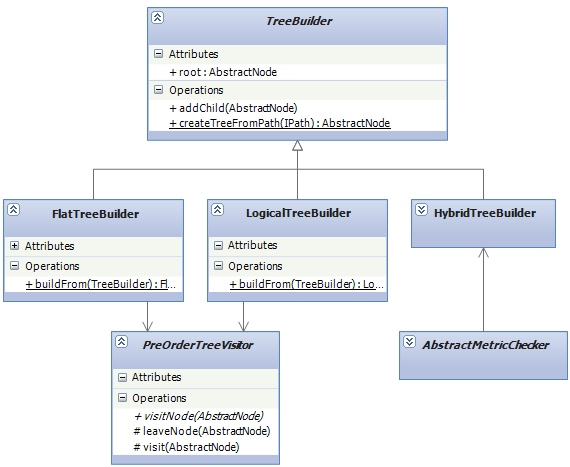
\includegraphics[width=\textwidth]{figures/model_treebuilder.png}
\end{center}
\caption{Class diagram with classes related to \textit{TreeBuilder}.}
\label{fig:model_treebuilder}
\end{figure}

\subsection{AbstractNode}
As illustrated in Figure~\ref{fig:model_tree} the \textit{AbstractNode} class is a simplified composite structure to hold all relevant data the view displays. Each node has one parent and any number of children. An \textit{AbstractNode} represents a file system object or an \textit{ASTNode}. The required information extracted from the \textit{ASTNode} are hold in a \textit{NodeInfo} instance. We extract the values from the \textit{ASTNode} instead of holding a reference to it so that the \textit{ASTNode} instance can be removed by the garbage collector. See chapter \ref{performance-tuning} for more details about related performance issues.

\begin{figure}[th]
\begin{center}
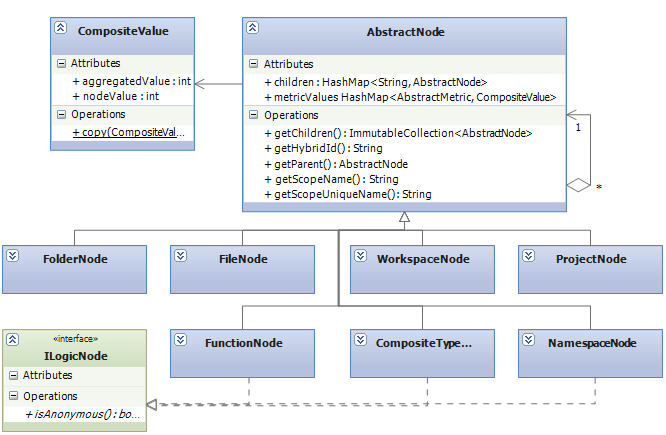
\includegraphics[width=\textwidth]{figures/model_tree.png}
\end{center}
\caption{Class diagram with classes related to \textit{AbstractNode}.}
\label{fig:model_tree}
\end{figure}

\subsubsection{AbstractNode Identifiers}
Each \textit{AbstractNode} has three types of string values that name it: hybridId, scopeName, scopeUniqueName. All of them are illustrated in Figure~\ref{fig:identifiers}.\\
The \textit{hybridId} is the tree wide unique identifier of a node. It is needed to identify the nodes and building the tree structures. The \textit{hybridId} is build by concatenating the \textit{scopeUniqueNames} of all ancestor nodes and its own \textit{scopeUniqueName}. To understand what a \textit{scopeUniqueName} is we first explain what a \textit{scopeName} is.\\
The \textit{scopeName} is the name of the represented underlying object. For instance the file name or the signature of a function. Logical nodes do not always have a name. For instance anonymous namespaces may exist at the same level. Hence it would be a problem to identify objects by using only their \textit{scopeName} because two namespaces at the same level with no name would have the same \textit{hybridId}.\\
Therefore we introduced the \textit{scopeUniqueName}. The \textit{scopeUniqueName} is build by appending the hash code of the \textit{NodeInfo} instance to the existing \textit{scopeName}.\\

Following example describes the identifier types used in \textit{AbstractNode} and is illustrated in Figure \ref{fig:identifiers}:
\begin{itemize}
\item \textbf{scopeName} of function \textit{f(int i)} is f(int i)
\item \textbf{scopeUniqueName} of an anonymous namespace is just a number (hash code)
\item \textbf{hybridId} of the function \textit{f(int i)} therefore is \\ Workspace:ProjectX:identifier\_test.cpp:2470869:A1338645:f(int i)2730475
\end{itemize}

\begin{figure}[th]
\begin{center}
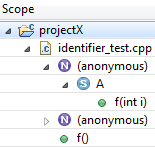
\includegraphics[scale=0.8]{figures/metriculator_hybrid_scope.png}
\end{center}
\caption{Sample tree structure}
\label{fig:identifiers}
\end{figure}

\subsubsection{CompositeValue}
The \textit{CompositeValue} is used by \textit{AbstractNode} objects to store the calculated values for each \textit{AbstractMetric}. As shown in Figure~\ref{fig:model_tree} the \textit{CompositeValue} is implemented as a pure value object.\\
The \textit{nodeValue} field stores the current value of the node. The \textit{aggregatedValue} field is calculated by the \textit{nodeValue} of it self plus the sum of all \textit{nodeValues} of its descendant nodes. The \textit{aggregatedValue} is calculated once when the Codan job finishes. Calculation is done for all nodes in the \textit{HybridTreeBuilder}. See chapter Performance Tuning \ref{performance-tuning} for more details.
An example which describes the \textit{CompositeValue} is illustrated in Figure \ref{fig:compositeValue_example}:\\

\begin{figure}[th]
\begin{center}
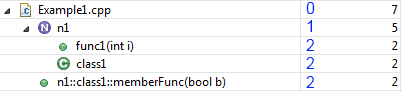
\includegraphics[scale=0.8]{figures/compositeValue_example.png}
\end{center}
\caption{Example of \textit{CompositeValue}, the values written in blue on the left are the node values and the other values on the right are the aggregated values.}
\label{fig:compositeValue_example}
\end{figure}

\subsection{TreePrinter}
The \textit{TreePrinter} class was mainly used for debugging purposes. We use it in our test cases to print the generated tree to the console after a test has been ran. Figure~\ref{fig:TreePrinter} shows a sample output. Scope names are trimmed to a maximum length and the metric values in each column are left aligned. The node values are in braces next to the aggregated values.

\begin{figure}[th]
\begin{center}
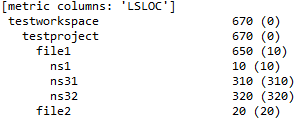
\includegraphics[scale=0.8]{figures/treeprinter_output.png}
\end{center}
\caption{Sample output of the \textit{TreePrinter} class.}
\label{fig:TreePrinter}
\end{figure}

\section{Metric Checkers}\label{checkers}
Codan offers extension points for third party tools to add new checkers. Metriculator uses Codan's extension points to define one checker per software metric. Every checker in metriculator inherits from the \textit{AbstractMetricChecker} that again inherits from the \textit{AbstractIndexAstChecker} of Codan.\\
Metriculator uses the \textit{AbstractMetric} class to encapsulate checkers and metric relevant data. Each checker implementation is associated with one \textit{AbstractMetric} implementation. When the checker is created on application start up it associates itself with the corresponding metric instance. A list of all \textit{AbstractMetric} instances is accessible through the plug-in singleton held by the \textit{MetriculatorPluginActivator}. See Figure~\ref{fig:metriculator_checker} for more details.

\begin{figure}[th]
\begin{center}
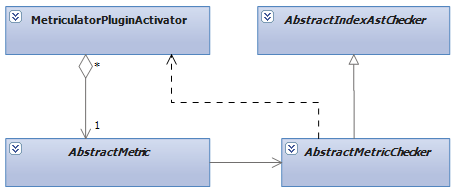
\includegraphics[]{figures/metriculator_checker.png}
\end{center}
\caption{Relations between the \textit{MetriculatorPluginActivator}, \textit{AbstractMetric} and \textit{AbstractMetricChecker} classes.}
\label{fig:metriculator_checker}
\end{figure}

Beside the checker reference \textit{AbstractMetric} implementations are responsible to implement a value aggregation strategy. The \textit{AbstractMetric} class provides a default aggregation strategy as you can see in Listing~\ref{aggregation_strategy_default}.

\begin{lstlisting}[style=C++0x, caption=Code snippet of the default value aggregation strategy implemented in \textit{AbstractMetric}, label=aggregation_strategy_default] 
public int aggregate(AbstractNode node){
	CompositeValue metricValue  = node.getValueOrDefaultOf(getKey());
	metricValue.aggregatedValue = 0;

	for(AbstractNode child : node.getChildren()) {
		metricValue.aggregatedValue += aggregate(child);
	}

	metricValue.aggregatedValue += metricValue.nodeValue;

	return metricValue.aggregatedValue;		
}
\end{lstlisting}

\subsection{Tasks}
Each \textit{AbstractMetricChecker} implementation is responsible for the following tasks:
\begin{itemize}
\item Visiting of the AST using a \textit{ScopedASTVisitor}. see \ref{ast_visitors}
\item Initialisation of its profile preferences
\item Problem creation and reporting
\end{itemize}

The following tasks are taken care of by the \textit{AbstractMetricChecker} class:
\begin{itemize}
\item Getting the hybrid tree model. see \ref{treebuilder}
\item Creating the file and folder nodes for each processed file and adding it to he hybrid tree model. see also \ref{processing}
\item Resetting its problems, all tree models and \textit{AbstractNode} references as soon as Codan has finished its job.
\end{itemize}

\subsection{Scope Listeners}\label{scopelisteners}
The \textit{IScopeListener} interface allows metric checkers to register themselves at \textit{ScopedAstVisitor} instances to be notified if the scope changes. Checkers for instance use this mechanism to report problems after function or type nodes have been analysed.\\
See Figure~\ref{fig:checkers} to see the environment of the \textit{AbstractMetricChecker} class.

\begin{figure}[th]
\begin{center}
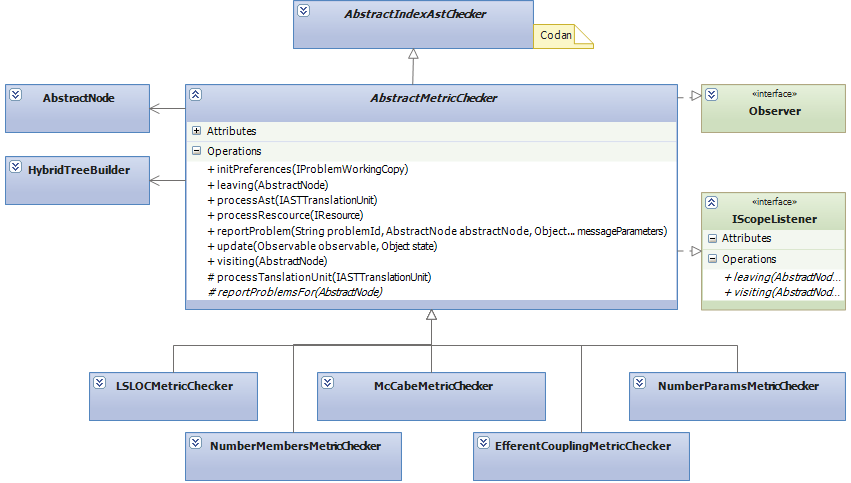
\includegraphics[width=\textwidth]{figures/checkers.png}
\end{center}
\caption{Class diagram with classes related to \textit{AbstractMetricChecker}}
\label{fig:checkers}
\end{figure}

\subsection{AST Visitors}\label{ast_visitors}

The \textit{ScopedASTVisitor} is responsible for visiting the AST and has a reference to the current scope node which is a \textit{AbstractNode} instance. The \textit{ScopedASTVisitor} inherits from the \textit{ASTVisitor} of Codan and implements the visit and leave methods. In the \textit{ScopedASTVisitor} all relevant \textit{ASTNodes} of a file, provided by the calling checker instance, are visited and added as nodes to the hybrid tree model. Thus all logical nodes of the hybrid tree model are created with \textit{ScopedASTVisitor} classes.\\

\textit{ScopedASTVisitor} implementations like \textit{LSLOCScopedASTVisitor} are responsible for analysing the \textit{ASTNodes} relevant for the related metric. \textit{ScopedASTVisitor} create the node values for the specific metric in the current scope. There is always one \textit{ScopedASTVisitor} associated with one \textit{AbstractMetricChecker}. Visitors can also notify registered \textit{IScopeListener} instances if a scope is changing. See chapter \ref{scopelisteners} for more details.
\\\\
Figure~\ref{fig:scoped_ast_visitor} shows a class diagram of the \textit{ScopedASTVisitor} and related classes.

\begin{figure}[th]
\begin{center}
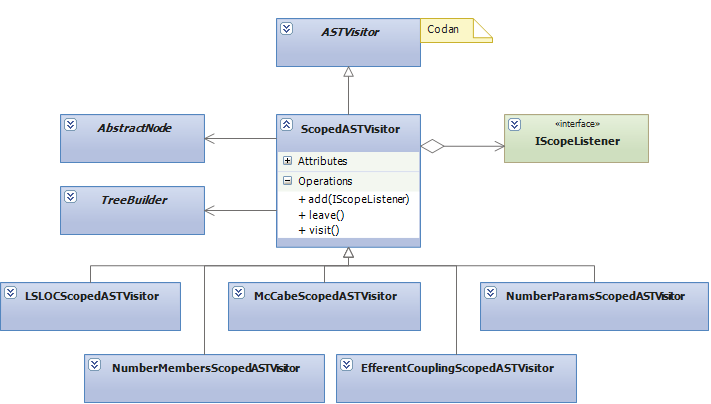
\includegraphics[width=\textwidth]{figures/scoped_ast_visitor.png}
\end{center}
\caption{Class diagram with classes related to \textit{ScopedASTVisitor}}
\label{fig:scoped_ast_visitor}
\end{figure}

\section{Processing}\label{processing}
The Codan framework invokes the metriculator checkers. At the end of the processing of Codan, the view of metriculator appears. The whole processing is described in detail below and is illustrated in Figure~\ref{fig:processing}.
\begin{enumerate}
\item A user runs Codan with the \textit{Run C/C++ Code Analysis} command in Eclipse CDT.
\item Metriculator is notified about the start of Codan.
\item Metriculator resets its models.
\item Codan starts processing the C++ resources to be analysed.
\item For each resource each checker is called to process it.
\item Each translation unit is processed.
\item The metriculator checker visits the relevant AST nodes to calculate metric data.
\item When Codan has finished, metriculator shows its view in Eclipse.
\end{enumerate}
\begin{figure}[hp]
 \centering
  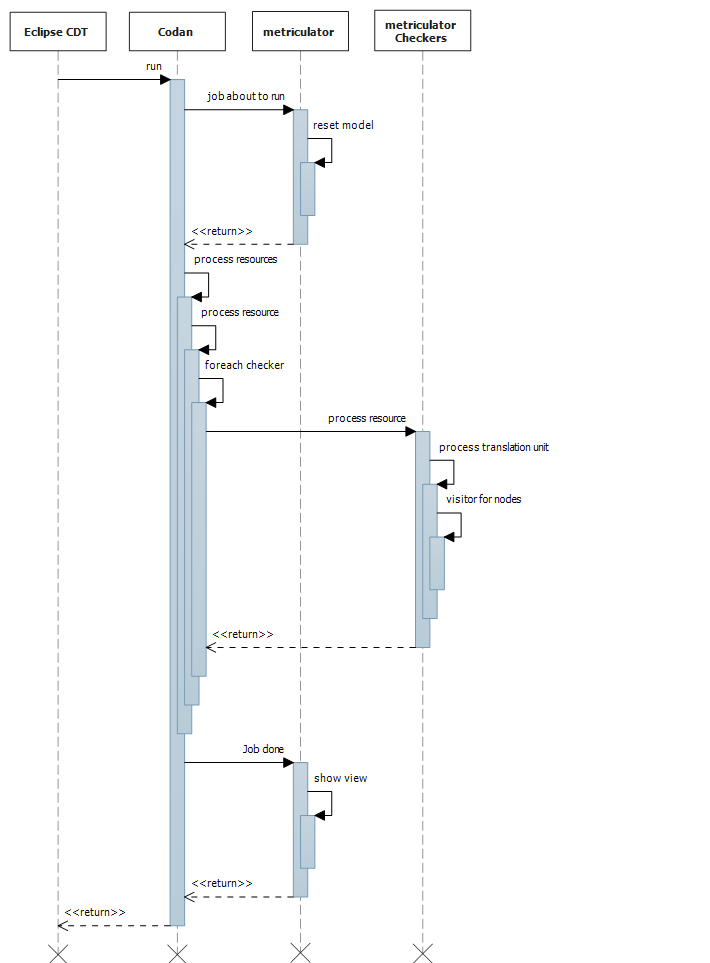
\includegraphics[width=\textwidth]{figures/processing.png}
 \caption{High level sequence diagram of the processing of metriculator}
  \label{fig:processing}
\end{figure}


\chapter{Conclusion}
Overall, we reached our basic objectives defined in chapter \ref{requirements}. The plug-in performs well in medium sized projects. It has a solid design and is easily extensible.\\
The following chapter describes analysis and problem finding processes related to performance issues. After that we describe the unresolved issues of the project. At the end we describe ideas to improve and extend metriculator.

\section{Performance Tuning}\label{performance-tuning}
In week nine we set up the last step in our deployment pipeline \cite{contdelivery}. That is the continuous and automated publishing of the latest plug-in build. The plug-in was made available through a publicly available p2 update site \cite{updatesite}. The update site allowed us to install the plug-in on an independent eclipse instance which is mandatory to test the performance.
According to the quantitative goals of this semester thesis \ref{Introduction} we ran our performance tests against the llvm project \cite{llvm} especially the clang sub project \cite{clang}.

The first manual test runs were very disappointing. The performance was very bad. Analysing two thousand LSLOC did work. Everything above was critical and most often eclipse ran out of heap space. Also the operation took very long to finish. We soon realized that for the remaining two weeks of development, performance tuning will have highest priority. The plug-in must perform well otherwise it would be useless, regardless of the number of features implemented.
Thanks to jprofiler \cite{jprofiler} we quickly figured out the time consuming methods and memory bottle necks.

\subsection{Timing Issues}
We first optimized metriculator to take less time of execution. This was mainly achieved by reducing the number of method calls by caching values instead of recalculating them on every request.
\\\\
An \textit{AbstractNode} is able to sum up all node values of its descendant nodes. This process has been triggered very often by the tree viewer control since every cell displays such an aggregated value. To fix that problem we now only aggregate the values once at the end of the code analysis, before the data are bound to the view.\\
Another hot spot was the clone mechanism of an \textit{AbstractNode}. Cloning was implemented as deep clone, which means that cloning one node in fact cloned the node itself and all descendant nodes. Before caching aggregation values this step was mandatory to show correct values in filter views. Thanks to cached values we changed the deep clone implementation to a shallow clone implementation. That is much more faster and saves even more memory.\\
Similar to the value aggregation problem was the path algorithm problem. Each \textit{AbstractNode} has a unique path that represents its position in the tree. The initial implementation requested the path of a parent node, every time a child was added. Since the path building algorithm was recursively it was very time and also memory consuming. Building the path only once and only force recalculation if mandatory solved that performance issue.

\subsection{Memory Issues}
The main reason why metriculator crashed at the beginning was because the huge amounts of memory allocation. The virtual machine run out of heap space and Eclipse crashed. We identified two problem areas.
\\\\
During the processing metriculator created ten thousands of char[] instances that allocated mega bytes of memory. We figured out that the instances were hold by C++ parser class instances that were used to create the AST. Since \textit{AbstractNode} referenced the \textit{ASTNode} instances they could not be removed by the garbage collector.\\
As a solution we introduced a new class called \textit{NodeInfo} that serves as pure value object holding only the relevant infos of an \textit{ASTNode} that we really need to keep. As a result memory allocation significantly decreased.\\
But there is still capability left to improve the memory allocation in \textit{NodeInfo}. We hold an \textit{IBinding} reference that allows us to merge function declaration and function definition. The merging task has to run after all checkers ran, because function declarations and definitions may be in different files. Since the problematic memory allocation happens during the processing we can not release the \textit{IBinding} references and that still causes a significant amount of memory being allocated.
\\\\
The second problem was caused by the jface \textit{TreeViewer} component. We used the \textit{TreeViewer} component in the hybrid view, as well as in all others views, including the filter view. But in the filter view, we never displayed hierarchical data but very large lists of for instance \textit{FunctionNodes}. The \textit{TreeViewer} component is not optimized to display flat lists. Therefore we decided to use the \textit{TableViewer} component in filter views. That decision tremendously improved the performance of the filter view mode. Now displaying and sorting thousands of \textit{FunctionNodes} just takes a fraction of a second. 
\\\\
The introduction of the \textit{TableViewer} component beside the existing \textit{TreeViewer} component forced us to create duplicated, almost identical code. Although their API is very similar, \textit{TreeViewer} and \textit{TableViewer} do not share a common base that we could use to create an abstract interface to interact with both of them. Additionally subclassing is not allowed in SWT \cite{swtsubclassing}. Therefore we just duplicated the code used for the \textit{TreeViewer} and replaced the types used.


\section{Known Issues}\label{knownissues}
There are some known issues that should be taken care of in future releases. This chapter describes this issues and also contains a reference to the issues documented in Redmine.

\subsection{Performance}
As already described in detail in section \ref{performance-tuning} we optimized metriculator to perform better on large input data. Currently metriculator can analyse about 300'000 physical lines of code if problem reporting is disabled and only the LSLOC metric is active. 
\\\\
Issue \#117 at http://sinv-56013.edu.hsr.ch/redmine/issues/117

\subsection{Zest Cloudio Integration}\label{zestcloudio}
The tag cloud integration is not stable yet. The code of this feature was taken from the project at \cite{sourcecloud_git} after the author contacted us and suggested to integrate his work. We just customized the code to work within metriculator. Generating a tag cloud based on large lists (for instance function nodes) sometimes results in exceptions saying that there is not enough drawing space available.
\\\\
Issue \#176 at http://sinv-56013.edu.hsr.ch/redmine/issues/176

\subsection{Installation via Composite Update Site}
When installing metriculator multiple steps are required in advance to install the prerequisites. Before metriculator can be installed via update site, users have to install CDT and the Zest framework separately. The current composite update site does not work.
\\\\
Issue \#177 at http://sinv-56013.edu.hsr.ch/redmine/issues/177

\subsection{Merging of Function Declarations in Anonymous Namespaces}
This bugs only relates to the logical view. If a function is declared in an anonymous namespace and the definition is outside of the anonymous namespace the definition does not replace the declaration. Instead the declaration and the definition are deleted.
\\\\
Issue \#166 at http://sinv-56013.edu.hsr.ch/redmine/issues/166


\section{Future Work}
There are many interesting not yet implemented metrics that would increase the value of metriculator, see chapter \ref{advobjectives} for an incomplete list.\\
Performance can further be improved to allow analysing source code with over about 300'000 physical lines of source code. Fixing that issue would make metriculator even more attractive to analyse large projects. Other unresolved issues are listed in chapter \ref{knownissues}.\\
A reasonable application of metriculator in the future is to serve as refactoring assistant. Based on a reported problem, metriculator could suggest a refactoring or quick fix that solves that problem.

\newpage
\thispagestyle{empty}
\mbox{}
\newpage


\appendix

\chapter{Environment Set up}
This appendix describes the hardware and software components that support us in reaching our project goals. We give detailed installation and configuration instructions and highlight problem areas to be aware of when setting up a similar environment.

\section{Hardware}
We use a virtual server to host different kinds of software that support us in our daily project tasks. The virtual server is hosted by the HSR. We have full root access and can connect to the server by VPN if we are outside of the \textit{HSR-LAN}. The server runs with Ubuntu 10.04 TLS on 1GB RAM. The host name is \texttt{sinv-56013.edu.hsr.ch}.

\section{Project Management Software}
To support our project management tasks we decided to use Redmine. The latest release at the start of our project was version 1.2.1. We use Redmine for the following tasks:
\begin{itemize}
\item issue tracking
\item time tracking
\item meeting records
\item Git repository browsing (login required)
\item Gather and share thoughts
\end{itemize}

Our Redmine instance is publicly and read only available at \url{http://tiny.cc/metriculator}.

\subsection{Set up \& Configuration}
We followed the set up instructions on \cite{redminesetup} to install and configure Redmine using Passenger.

Basically we used the following commands:
\begin{lstlisting}[style=console, caption=Redmine set up commands]
sudo aa-complain /usr/sbin/mysqld
sudo apt-get update
sudo apt-get install redmine redmine-mysql
sudo apt-get install libapache2-mod-passenger
sudo ln -s /usr/share/redmine/public /var/www/redmine
sudo a2enmod passenger
sudo chmod a+x /usr/share/redmine/public
sudo service apache2 restart
\end{lstlisting}

After these steps, Redmine is up and running at \texttt{http://host/redmine}.

To enable Redmine repository browsing the user under which Apache runs has to have read access to the Git root directory.
By default Apache runs as \textit{www-data}. Additionally, you might have to refresh Redmines repository cache.
\begin{lstlisting}[style=console, caption=Redmine repository browsing set up]
# preferably gather all users that require git access in one group
sudo adduser www-data group-with-read-access
cd /path/to/redmine && /usr/bin/ruby1.8 script/runner \
"Repository.fetch_changesets" -e production
\end{lstlisting}

\textbf{Caution:} Redmine version 1.2.x requires rails version 2.3.11 (with Ruby gems 1.3.7).\\
We also had to reset our MySQL root password. We followed the instructions on \cite{mysqlpasswordreset} to accomplish this.

\section{Version Control System, Git}
To support our file version management we decided to use Git. The latest release at the start of our project was version 1.7.6. We used the following commands to set up Git:
\begin{lstlisting}[style=console, caption=Git repository set up]
# login as root

#add a group for the git-users 
group="git-users"
groupadd "$group"

# add a user
user="name_of_user"
adduser "$user"

# add the user to the git group
usermod -aG "$group" "$user"

# shared directory for the git-repository
mkdir -pv /var/gitrepo
chmod 770 /var/gitrepo
chgrp "$group" /var/gitrepo
chmod g+s /var/gitrepo

# create a git repository
# --shared: all users of the group must have access
# --bare: no working directory, it is just the repository
cd /var/gitrepo
mkdir repository.git
cd repository.git

git init --bare --shared=group

# acces via ssh with public-key authentication
# every user has to generate a key
# linux: generates a private and a public key in ida_rsa.pub
ssh-keygen -t rsa -b 2048 -f ~/.ssh/id_rsa

# the public key of the users has to be installed on the server
umask 077
mkdir -v "/home/${user}/.ssh"
cat "id_rsa_${user}.pub" >> "/home/${user}/.ssh/authorized_keys"
chown "$user:$user" "/home/${user}/.ssh"
# "ida_rsa_${user}.pub" ist he public key of the user

# cloning the git repository
git clone ssh://user@host/var/gitrepo/repository.git
\end{lstlisting}

\textbf{Caution:} For using Git on Windows and how to set up the required SSH access see \cite{wingitsetup}.

\section{Development Environment}\label{devenv}
The plug-in was developed in Eclipse Indigo using the plug-in development environment (PDE) plug-in. To test metriculator we used sample C++11 source code. To force the compiler to build according to the C++11 standard add the \texttt{-std=gnu++0x} flag to the following field: \textit{Project Properties > C/C++ Build > Settings > GCC C++ Compiler > Miscellaneous > Other flags}.

\section{Continuous Integration Server}
We installed Jenkins 1.434 \cite{jenkinssetup} as continuous integration server. Jenkins provides a solid platform for various plug-ins that enhance its basic continuous integration features. Our Jenkins instance requires the plug-ins listed in table \ref{jenkins_plugins}.

\begin{table}[th]
\begin{center}
\begin{tabular}{|l|l|p{.4\textwidth}|}
\hline
Name & Version & Description \\
\hline
Maven 2 Project & 1.430 & Allows to trigger Maven goals on build events. \\
Static Analysis Utilities & 1.30 & Provides utilities for the static code analysis plug-ins. \\
Static Analysis Collector & 1.17 & This plug-in is an add-on for the plug-ins Checkstyle, Dry, FindBugs, PMD, Tasks, and Warnings: the plug-in collects the different analysis results and shows the results in a combined trend graph.\\
FindBugs plug-in & 4.29 & This plug-in collects the FindBugs analysis results of the project modules and visualizes the found warnings. \\
Hudson Xvnc & 1.10 & Allows projects to run Xvnc during a build. Xvnc is required to run CDT plug-in tests since they start Eclipse. \\
Jenkins GIT &	1.1.12 & Integrates Git with Jenkins. \\
Jenkins Emma & 1.25 & Integrates EMMA code coverage reports to Jenkins.\\
ChuckNorris & 0.4 & Displays a picture of Chuck Norris followed by enlightening statements. \\
\hline
\end{tabular}
\caption{Installed Jenkins plug-ins}
\label{jenkins_plugins}
\end{center}
\end{table}

With Jenkins in place we can always monitor the health of our latest commits. For example if some unit tests fail, Jenkins will report that on the project homepage.

\subsection{Set up \& Configuration}
To set up Jenkins we followed the set up instructions on \cite{jenkinssetup}. Basically we used the following commands:\\
\begin{minipage}[t]{\textwidth}
\begin{lstlisting}[style=console, caption=Jenkins set up commands]
sudo aptitude install openjdk-6-jre
wget -q -O - http://pkg.jenkins-ci.org/debian/jenkins-ci.org.key | \
sudo apt-key add -
sudo sh -c 'echo deb http://pkg.jenkins-ci.org/debian binary/ > \
/etc/apt/sources.list.d/jenkins.list'
sudo aptitude update
sudo aptitude install jenkins
\end{lstlisting}
\end{minipage}

\section{Build and Deployment Automation}
The CDT project supports ant and Maven as build automation platform. We decided to give Maven (in contribution with Tycho) a try because it seemed a lot easier to maintain and has already been used in recent projects at HSR.

\subsection{Set up \& Configuration for Windows}\label{mavenwindows}
Since we have never used Maven before, we started using Maven on the local development environment. It was not mandatory to do something locally, but it simplified to get in touch with Maven for the first time. We first set up the initial configuration files for our projects. We followed the following steps to set up Maven on our Windows development machines:

\begin{itemize}
\item Download Maven from \cite{mavendownload} and extract archive to <target>
\item Add <target>\textbackslash bin to the PATH variable
\item Open your command line, change to your projects root directory.
\item Run\\\texttt{run mvn org.codehaus.tycho:maven-tycho-plugin:generate-poms \
\\-DgroupId=ch.hsr.ifs.cdt.metriculator 
\\-Dtycho.targetPlatform=C:\textbackslash Programme\textbackslash eclipse}
\\Where targetPlatform should point to your Eclipse installation folder.
\\ This command will generate or update pom.xml files in all directories in your project root. Chapter \ref{mavenxml} explains how to customize this pom.xml files.
\end{itemize}

\subsection{Set up \& Configuration for Ubuntu}
Follow the steps on \cite{mavenubuntusetup} to install Maven 3 on Ubuntu. Basically these are the steps:

\begin{lstlisting}[style=console, caption=Maven set up commands]
sudo mkdir /usr/local/apache-maven
cd /usr/local/apache-maven/
sudo wget http://ftp.heanet.ie/mirrors/www.apache.org/dist/ \
maven/binaries/apache-maven-3.0.2-bin.tar.gz
tar -xzvf apache-maven-3.0.2-bin.tar.gz
\end{lstlisting}

After that make sure to configure the environment variables as described at \cite{mavenubuntusetup}.
\\\\
Our plug-in unit tests require Maven to execute headless builds. That for we have to install Xvnc with a X11 window manager. Use the following commands to install Xvnc as virtual screen buffer and metacity as window manager.

\begin{lstlisting}[style=console, caption=Set up xvnc]
sudo aptitude install vnc4server metacity
sudo su jenkins
vncserver
# enter password manually
\end{lstlisting}

After the install command we have to manually set the vncserver password for the Jenkins user. Otherwise the Jenkins build will fail because no password has been set.

\subsection{Maven XML Configuration}\label{mavenxml}
Maven uses pom.xml for build instructions. We have one pom.xml in the root directory of all Eclipse projects (root pom) and one in each subdirectory (project pom). To automatically generate an initial version of the pom files follow the instructions in chapter \ref{mavenwindows}. All pom files are checked-in to the VCS as well. This chapter only highlights the changes applied to the generated pom files.
\begin{description}

\item[Version]
The version tag in all pom files should specify the same version as your plug-in manifest does. We use \texttt{<version>0.0.1.qualifier</version>} in the project pom files and \texttt{Bundle-Version: 0.0.1.qualifier} in our plug-in manifests.\\
All project pom files refer to the root pom file. The reference contains a version tag as well. The version tag of the root pom and the version referenced in the project pom files have to match. We use \texttt{<version>0.0.1-SNAPSHOT</version>}.

\item[Repositories]
Although we imported some CDT projects into our Eclipse workspace (see chapter \ref{devenv}) there is no need for Maven to build them all. The only modules that Maven has to build are the metriculator projects. Maven knows how to resolve the dependencies of our projects and may download them from remote repositories. We only need to specify the repositories to search in our root pom.

\begin{lstlisting}[style=Xml, caption=Maven repositories]
<repositories>
       <repository>
         <id>cdt-indigo</id>
		 <!-- required to resolve cdt.core.tests dependencies of test project 
		 (in eclipse we use the project 'testing-project'
		 that provides required jar files) -->
         <url>http://download.eclipse.org/tools/cdt/updates/indigo</url>
         <layout>p2</layout>
       </repository>
	   <repository>
         <id>indigo</id>
         <url>http://download.eclipse.org/releases/indigo</url>
         <layout>p2</layout>
	    </repository>	
		<repository>
         <id>updates</id>
         <url>http://download.eclipse.org/eclipse/updates/3.7</url>
         <layout>p2</layout>
		</repository>	
		<repository>
		 <!-- indigo swtbot release not available yet, 14.nov.2011 -->
         <id>swtbot</id>
         <url>http://download.eclipse.org/technology/swtbot/helios/ \
              dev-build/update-site</url>
         <layout>p2</layout>
       </repository>
	   <repository>
         <id>zest</id>
         <layout>p2</layout>
         <url>https://hudson.eclipse.org/hudson/job/gef-zest-integration \
         /ws/org.eclipse.zest.repository/target/repository/</url>
      </repository>	   
	</repositories>
\end{lstlisting}

\textbf{Caution:} Note that at the time of writing the latest swtbot release available is the one for helios.

\item[Target Platform]
Since we want Maven to be able to build on Windows machines as well as on our Linux based CI server we had to define different target platforms in our root pom. We use Tycho in version 0.10.0.
\begin{lstlisting}[style=Xml, caption=Maven target platform configuration]
<groupId>org.sonatype.tycho</groupId>
<artifactId>target-platform-configuration</artifactId>
<version>${tycho-version}</version>
<configuration>
   <resolver>p2</resolver>
   <environments>
     <environment>
        <os>win32</os>
		<ws>win32</ws>
		<arch>x86</arch>
     </environment>
     <environment>
		<os>linux</os>
		<ws>gtk</ws>
    	<arch>x86_64</arch>
     </environment>
  </environments>
</configuration>
\end{lstlisting}

\end{description}

\subsection{Jenkins Maven Integration}
There is a Maven plug-in available for Jenkins. This plug-in wraps the \texttt{mvn} command of Maven. But it is also possible to use a custom build script that invokes the \texttt{mvn} command. Since our build requires other actions being executed prior to the Maven build we use a custom build script. Another advantage of such a script is, that it is easier to maintain. All build steps are saved in one place and easy to change.

\begin{lstlisting}[style=console, caption=Jenkins build script]
#!/bin/sh

export PATH=/usr/local/apache-maven/apache-maven-3.0.3/bin:$PATH
#make $DISPLAY (from xvnc) globally available so that
#other processes can access it.
export DISPLAY=$DISPLAY
THIS=$(readlink -f $0)
BUNDLE_ROOT="`dirname $THIS`"

cd $BUNDLE_ROOT
mvn -e clean install
\end{lstlisting}

\chapter{Metriculator Metrics}
This chapter describes the results of a metric analysis applied to the metriculator plug-in source code.

\section{Finding Problems using FindBugs}
FindBugs did not find any problems.

\section{Static Source Code Analysis}
We used the Eclipse metrics plug-in  \cite{metrics_plugin} to analyse the metriculator source code. 
\subsection{Warnings}
The analysis found two warnings, both are related to the McCabe metric.\\
The method \textit{LSLOCScopedASTVisitor.visit(IASTStatement)} has a McCabe value of 16 which is 6 above the threshold of 10. Since this method has already been refactored heavily and reviewed by our supervisor we decided not to change the current implementation.\\
The method \textit{NodeInfo.equals(Object)} has a McCabe value of 14 which is 4 above the threshold of 10. Since we have many fields to compare the McCabe value is exceptionally high. Based on the best practice patterns \cite{jiaei_equals} we used in our implementation we do not think it would make much sense to further refactor the method.

\subsection{metriculator Metrics Applied to Itself}
This section outlines the metric results of the metrics that both the metrics plug-in and metriculator implement. The metrics plug-in does not always use the exact same metric names as metriculator does, but they can easily be mapped to the names we used.
\begin{description}
\item[Method Lines of Code (LSLOC)] Beside the code in the tag cloud component, which we did not change (details at \ref{zestcloudio}), the method \textit{MetriculatorPluginActivator.showMetriculatorView()} has the most lines of code, namely 40. This is because we create an anonymous class that implements an interface with plenty of methods. Since there is no adapter for that interface we have to implement all the methods, although we just need one.\\
The test package has 1410 lines of code. All other packages (views, resources, checkers, metriculator, model.*) together count 3559 lines of code.
\item[Efferent Coupling] The highest efferent coupling on package level is 15, for the package ch.hsr.ifs.metriculator.checkers. This package has many references to the model packages.
\item[Number of Parameters] The highest value is 4 which is good enough.
\item[Number of Attributes (Number of Members per Type)] The class \textit{MetriculatorView} has the highest value of 22.
\end{description}

\section{Dependecy Analysis}
We used Structure101 to analyse the architecture of metriculator. As visible in Figure~\ref{fig:structure101} Structure101 detected eleven cyclomatic dependencies between the model and the metriculator package. Nine out of this eleven dependencies are because the \textit{AbtractMetricChecker} class requires to use the plug-in singleton. The remaining two dependencies also come from the \textit{AbstractMetricChecker} class. Metric checkers register itself as job listener to be notified when the Codan command is about to run or has finished. This events are mandatory to trigger for example post execution actions like value aggregation.

\begin{figure}[th]
\begin{center}
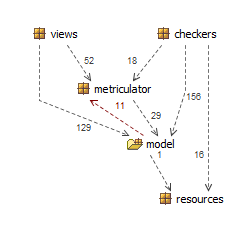
\includegraphics[scale=0.5]{figures/structure101_composition.png}
\end{center}
\caption{Dependency graph of metriculator generated by Structure101.}
\label{fig:structure101}
\end{figure}

\section{Test Coverage}
We used the EclEmma plug-in for Eclipse \cite{emma} to analyse the code coverage after running all unit test. The coverage results are shown in Figure~\ref{fig:emma}. The left column contains the packages and files analysed, the right column numbers the test coverage in percent. The elements of our interest are expanded and will be explained in this section.
\\\\
\subsection{UI Code}
The packages mainly dedicated to the view have a low test code coverage. This is because we do not have ui test code. Following packages heavily contain code that is related to the view: views, resources, tagcloud.*.\\
The \textit{AbstractNode} implementations in the package model.nodes all have a coverage of over 50\%. The reason for this low coverage in some classes is because they all implement the \textit{AbtractNode.getIconPath()} method which is only called from the view. Also the \textit{AbstractMetricChecker} has 7 out of 15 methods that are only called if the view is run.

\subsection{Model Code}
The checkers and model packages have a test coverage of over 80\%. Most units tests validate the correctness of the checker implementations which is reflected in a 95\% coverage of the checker package.\\

\begin{figure}[th]
\begin{center}
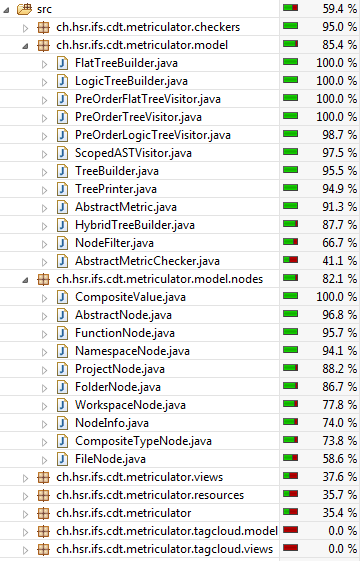
\includegraphics{figures/emma_coverage.png}
\end{center}
\caption{Screenshot of the emma code coverage analysis after running all unit tests.}
\label{fig:emma}
\end{figure}

\chapter{User Manual}
This user manual explains developers familiar with Eclipse and C++ how to use metriculator. It assumes that Eclipse CDT is already installed.

\section{Installation}
\begin{enumerate}
\item Install the Zest framework via update site from: \\ https://hudson.eclipse.org/hudson/job/gef-zest-integration/ws/org.eclipse.zest.repository/ \ target/repository/ (see Figure \ref{fig:zest_install})
\begin{figure}[th]
\begin{center}
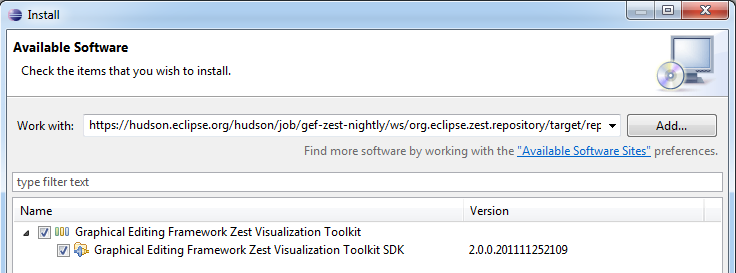
\includegraphics[scale=0.5]{figures/zest_install.png}
\end{center}
\caption{Use the wizard at \textit{Help > Install New Software \ldots}}
\label{fig:zest_install}
\end{figure}
\item Install metriculator via update site from:\\
 http://sinv-56013.edu.hsr.ch/updatesite/site (see Figure \ref{fig:metriculator_install})
\begin{figure}[th]
\begin{center}
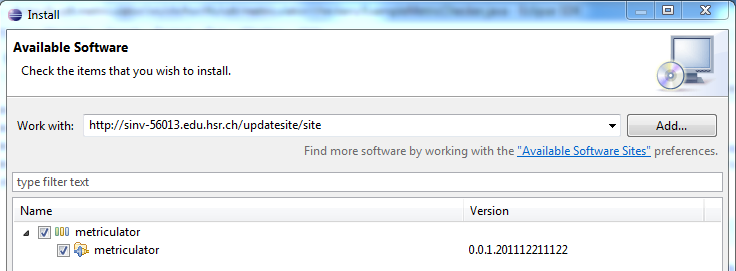
\includegraphics[scale=0.5]{figures/metriculator_install.png}
\end{center}
\caption{Use the wizard at \textit{Help > Install New Software \ldots}}
\label{fig:metriculator_install}
\end{figure}
\end{enumerate}
\section{Start code analysis with metriculator}
\begin{enumerate}
\item Choose your C++ source code to be analysed. Select one or more files and folders.
\item In the Project Explorer right click on the selection. This can be one or more projects, folders and files. Then choose to run the command \textit{Run C/C++ Code Analysis}. This will start the static code analysis and metriculator will analyse the source code with the activated metrics. After the analysis the metriculator view opens.
\end{enumerate}

\section{Configuration of metriculator}
\begin{enumerate}
\item Open the Eclipse preferences via \textit{Window > Preferences}
\item Open the Code Analysis preferences for C/C++ (see Figure \ref{fig:preferences})
\begin{figure}[th]
\begin{center}
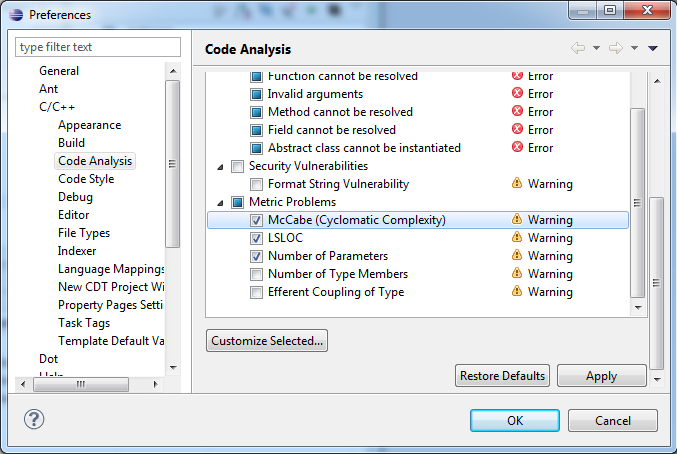
\includegraphics[scale=0.5]{figures/preferences.png}
\end{center}
\caption{metriculator checker preferences}
\label{fig:preferences}
\end{figure}
\item Under \textit{Metric Problems} you can enable or disable metrics you want to run (see Figure \ref{fig:preferences})
\item Double click on a metric to open the metric preferences dialog.
\item Specify the thresholds for the metrics (see Figure \ref{fig:problem})
\item Activate / Deactivate problem reporting with problem markers (see Figure \ref{fig:problem}). If you deactivate the problem reporting, the metriculator view will still highlight problematic cells, but the problem will not be reported to the Eclipse \textit{Problems View}. That implies that no markers are created in source code editors.
\begin{figure}[th]
\begin{center}
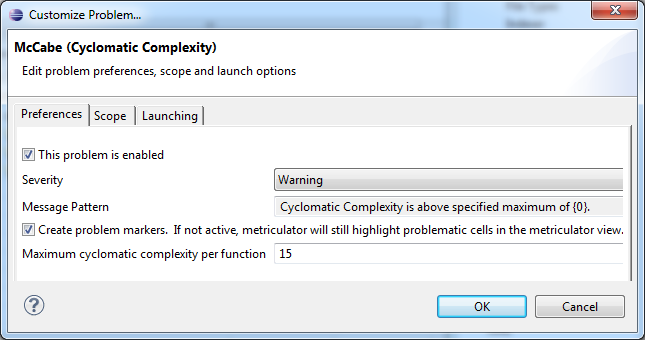
\includegraphics[scale=0.5]{figures/problem.png}
\end{center}
\caption{Customise Problem}
\label{fig:problem}
\end{figure}
\end{enumerate}

\section{Working with the Views}\label{the_views}
Use the different views to watch at the results. That helps you detect problems and obtain an overview of the quality and size of the analysed source code. 
Different metriculator views show the metric values from different perspectives. In all views all columns can be sorted. Cells with metric values beyond the thresholds are highlighted, this helps figuring out potential problems in your source code. All scope labels, for example a function name, can be double clicked to open an eclipse editor with the file where the function is in and to select the function code. Views with a tree view (hybrid view and logical view) can be easily expanded and collapsed with the commands in the upper right corner of the metriculator view.

\subsection{View Types}
\begin{itemize}
\item hybrid view (Figure \ref{fig:hybrid_view_manual})
\begin{figure}[th]
\begin{center}
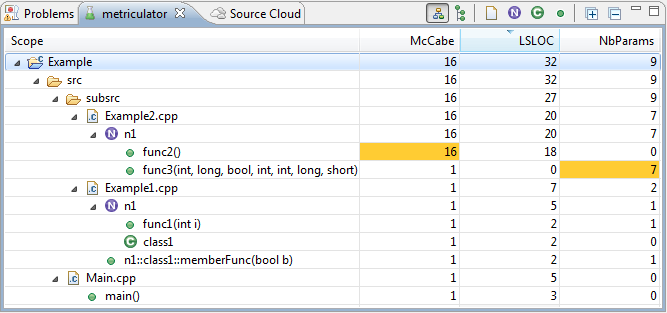
\includegraphics[scale=0.8]{figures/hybrid_view.png}
\end{center}
\caption{Hybrid view - This is the default view. It shows the projects and its content as a mix of physical and logical nodes in a tree structure.}
\label{fig:hybrid_view_manual}
\end{figure}
\item logical view (Figure \ref{fig:logical_view_manual})
\begin{figure}[th]
\begin{center}
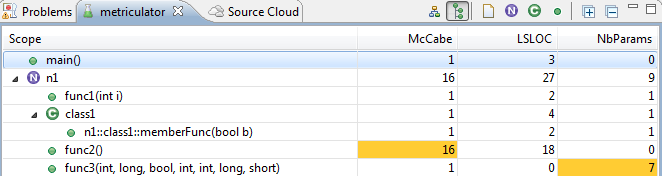
\includegraphics[scale=0.8]{figures/logical_view.png}
\end{center}
\caption{Logical view - Shows the logical representation of the source code in a tree structure. The logical elements like namespaces or classes are decoupled from the physical location and merged together.}
\label{fig:logical_view_manual}
\end{figure}
\item filter view (Figure \ref{fig:filtered_functions_view_manual})
\begin{figure}[th]
\begin{center}
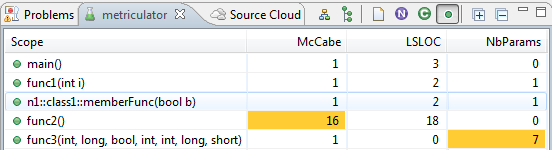
\includegraphics[scale=0.8]{figures/filtered_functions_view.png}
\end{center}
\caption{Filter view - Shows a filtered representation of the hybrid view. Possible filters are files, namespaces, types and functions.}
\label{fig:filtered_functions_view_manual}
\end{figure}

\item tag cloud (Figure \ref{fig:tag_cloud_lsloc})
\begin{figure}[th]
\begin{center}
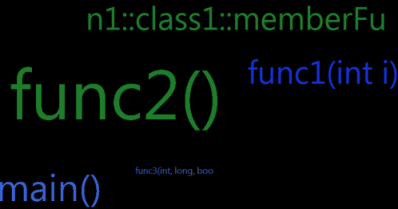
\includegraphics[scale=0.8]{figures/tag_cloud_lsloc.png}
\end{center}
\caption{Tag cloud - visualisation of the nodes for a specific metric. The higher the metric value the bigger the font size of the name in the cloud. This tag cloud was generated for the metric LSLOC.
}
\label{fig:tag_cloud_lsloc}
\end{figure}
\end{itemize}

\section{Problem Reporting and Markers}
Metriculator allows to report problems to the Problems View built-in Eclipse. This will also set markers in source code editors next to the problematic source code sections. If the option \textit{Create problem markers} in the metric problem preferences is activated (see Figure \ref{fig:problem}), metriculator reports the problems (Example \ref{fig:problems_view_manual}) and sets the markers (Example \ref{fig:marker_manual}). Otherwise the problems are just visible inside the metriculator view. Cells with problematic values are highlighted anyway.\\
\textbf{Hint}: Deactivating problem reporting can improve the speed of the analysis. \cite{eclipse_errrep_slow}.
\begin{figure}[th]
\begin{center}
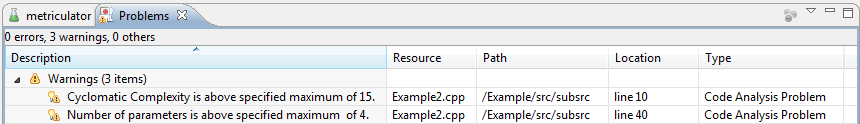
\includegraphics[scale=0.75]{figures/problems_view.png}
\end{center}
\caption{Problems View}
\label{fig:problems_view_manual}
\end{figure}

\begin{figure}[th]
\begin{center}
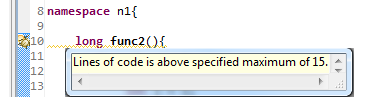
\includegraphics{figures/marker.png}
\end{center}
\caption{Problem marker in the source code editor with a message explaining the problem.}
\label{fig:marker_manual}
\end{figure}


\chapter{Developer Manual}
Metriculator allows you to add new C++ metrics easily. There are already some metrics implemented which might help you to implement additional metrics. The following steps describe how you can add new metrics fast an simple.
This manual assumes that you are working with Eclipse and have installed the Plug-in Development Environment (PDE) as well as the C/C++ Development Tooling (CDT) plug-in.

\section{Set up}
\begin{enumerate}
\item Checkout sources from the Git repository at sinv-56013.edu.hsr.ch/var/gitrepo/metricular.git.
\item In Eclipse \textit{Import Existing Projects into Workspace}, select the repository checked out from point 1.
\item Set the missing baselines to \textit{ignore} in \textit{Eclipse > Window  > Preferences > Plug-in Development > API Baselines}
\item Open the target file in the package metriculator and set it as target platform (illustrated in Figure \ref{fig:target_manual})
\item Update all the locations (illustrated in Figure \ref{fig:target_manual})
\begin{figure}[th]
\begin{center}
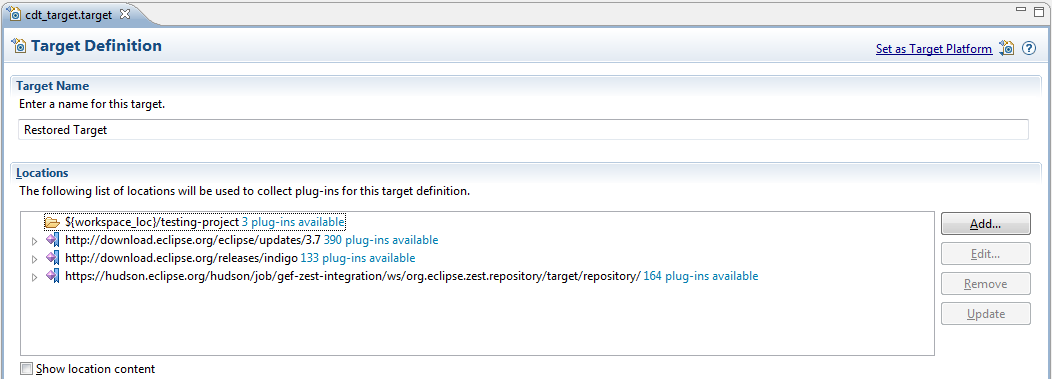
\includegraphics[scale=0.5]{figures/target.png}
\end{center}
\caption{Target file}
\label{fig:target_manual}
\end{figure}
\item Clean all projects if there are still errors
\end{enumerate}

\section{Adding a new Metric}
\begin{enumerate}
\item Add a new checker with a problem in the plugin.xml. (illustrated in Figure \ref{fig:pluginxml})
\begin{figure}[th]
\begin{center}
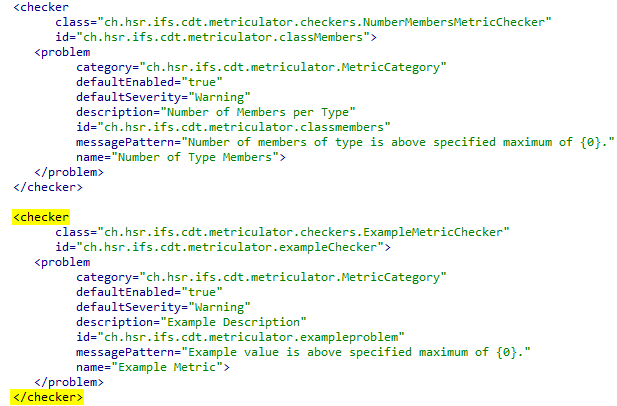
\includegraphics[scale=0.75]{figures/pluginxml.png}
\end{center}
\caption{Part of the plugin.xml file. The highlighted element is the newly added checker.}
\label{fig:pluginxml}
\end{figure}
\item Create a new metric class which inherits from \textit{AbstractMetric} class.
\begin{enumerate}
\item If your new metric requires a non default metric value aggregation override the \textit{aggregate} method
\end{enumerate}
\item Create a new metric checker class that inherits from \textit{AbstractMetricChecker}.
\begin{enumerate}
\item Define a problem ID.
\item Create the name, description and preferences strings.
\item Add the name, description and preferences strings to the \textit{MetricLabels.properties} file in the package resources.
\item Add the name, description and preferences strings to the \textit{MetricLabels} class.
\item Create a new instance of the metric in this checker.
\item Register the new metric at the \textit{MetriculatorPluginActivator} singleton instance.
\item Implement the \textit{reportProblemsFor} method.
\item Implement the \textit{processTranslationUnit} method. See chapter 3 for further information about visitors.
\end{enumerate}
\item Create a new \textit{ScopedAstVisitor}.
\begin{enumerate}
\item Define the \textit{key} string for this metric.
\item Override the \textit{shouldVisitxxx} fields to visit the desired AST nodes.
\item Override and implement the \textit{visit} method for the desired AST nodes to be visited (could be one or more visit methods).
\end{enumerate}
\end{enumerate}

\section{Writing Checker Tests}
Each checker has its own test class. When implementing a new checker test you should be aware of the following:

\begin{itemize}
\item Add your test class to the test suite by modifying AllTests.java
\item You can use the \textit{TreePrinter} class to print a tree structure to the console
\item Use the \textit{loadCodeAndRun(getAboveComment())} methods provided by Codan, to define the C++ code your checker under test will use.
\item Reset the model after each test method has been ran.
\end{itemize}

\chapter{Project Management}
This chapter provides an overview to project management related tasks such as project planning and spent time analysis.
\section{Project Plan}
The project lasts fourteen weeks from September 19. to December 23. 2011. The first version of the project plan \ref{fig:schedule_start} was created in week one. During the first seven weeks the initial project plan has experienced a few minor changes \ref{fig:schedule_end}.


\begin{figure}[h!tbp]
  \centering
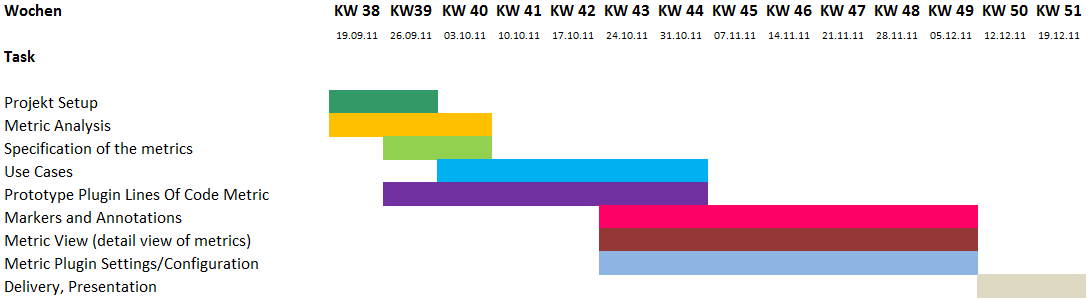
\includegraphics[width=\textwidth]{figures/schedule_start.png}
\caption{Initial version of the project plan.}
\label{fig:schedule_start}
\end{figure}

\begin{figure}[h!tbp]
  \centering
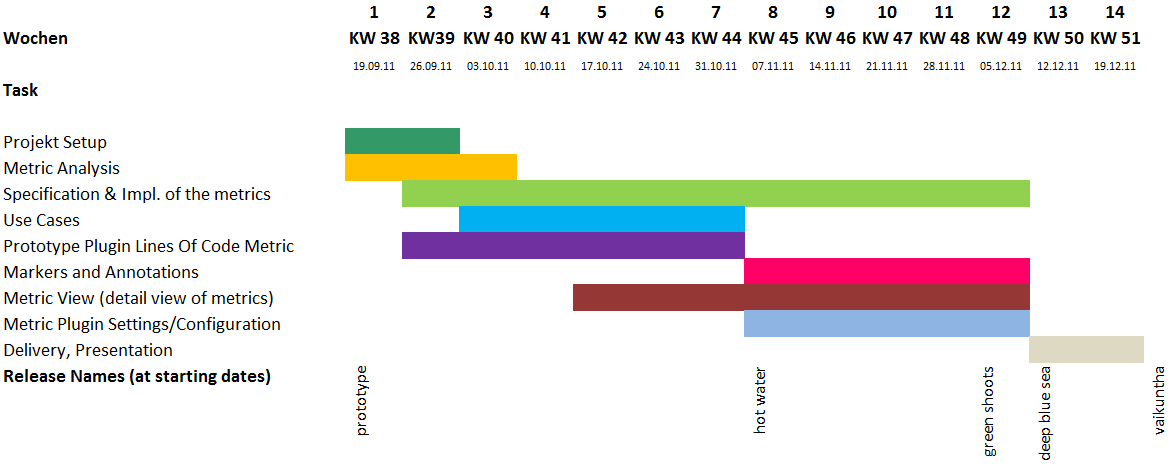
\includegraphics[width=\textwidth]{figures/schedule_end.png}
\caption{Final version of the project plan.}
\label{fig:schedule_end}
\end{figure}


The task \texttt{Specification of metrics} has been renamed to \texttt{Specification \& Impl. of metrics}. As we started with the implementation of the first metric (\ref{lsloc}) we noticed that there was no task on the project plan for metric implementation. We did not create a new one instead we extended the existing specification task since specification and implementation can not strictly be separated especially because we follow iterative development cycles.\\
The second change is related to user interface tasks. They were initially planned to start in week 43, two weeks before the release of the prototype. In week 41 we gladly realized that we are on schedule and that it would be reasonable to start with the implementation of the view one week earlier as planed. As we started with the view we decided to shift the markers and settings tasks to the end of the prototype phase because they were relatively easy to implement since the Codan framework provides a simple API to handle them.

\section{Time Schedules}
This chapter evaluates the time spent during the project. The first section describes the time spent per project member and week, the next section the time spent on each reported bug.

\subsection{Spent Time per Project Member}
Figure~\ref{fig:spenttime} shows the time spent per member. The semester thesis module is worth 8 ECTS. This means that the expected work per week of an average student to pass the module is about 17 hours\footnote{8 ECTS * 30 hours per ECTS / 14 weeks}. In average each of us worked about 295 hours in total, which is 57 hours (24\%) above the expected 238 hours.
\begin{figure}[h!tbp]
  \centering
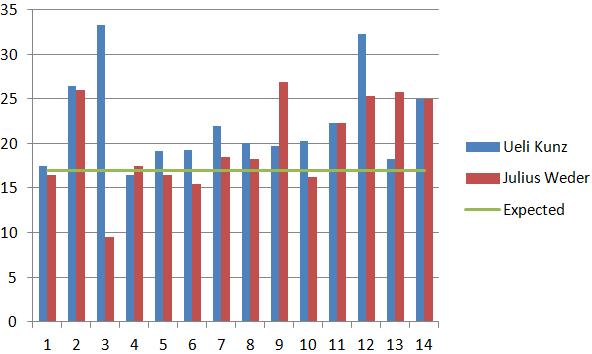
\includegraphics[width=\textwidth]{figures/spenttime.png}
\caption{Time spent per member working on the project.}
\label{fig:spenttime}
\end{figure}

\subsection{Mean Time to Fix}
The mean time to fix Figure \ref{fig:mttf} shows how long it took to fix a bug after it was reported.
\begin{figure}[h!tbp]
  \centering
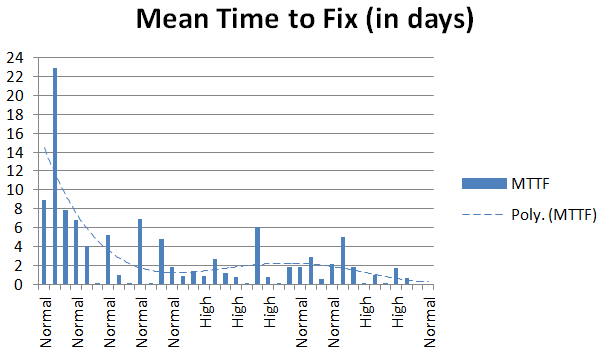
\includegraphics[width=\textwidth]{figures/mttf.png}
\caption{Number of days it took to fix bugs after they were reported. X axis is sorted ascending by date.}
\label{fig:mttf}
\end{figure}

The second bug has the biggest MTTF. This bug was reported because the Jenkins server was not accessible from outside the HSR LAN. Since this circumstance was not critical for us to go on working, we did not prioritize it. All other bugs were fixed within maximum nine days.

\section{Personal Impression}
From the very beginning of this project we both worked consequent and targeted to create a highly useful and simple to understand plug-in. In the sub chapters of this section each team member writes about his personal impressions during this project.\\
But first of all we would like to thank our advisor, Prof. Peter Sommerlad, for his valuable time and competent advices. Special thanks goes to Thomas Corbat, who was always ready to generously assist us at technical problems.

\subsection{Ueli Kunz}
At the start of this project I was very excited what will be the outcome. I was highly motivated to deliver a well designed and stable plug-in. Although it was a small team, I was also interested in gathering more project management experiences and applying the lessons learned from earlier term projects. Getting to known with a new framework and contributing to it was also a motivating task. Since I have already benefited from other open source projects I have been willing to give something back.
\\\\
At the beginning we had some extra effort setting up the project environment software. Setting up Jenkins with Git and Redmine was worth the experience but I think next time it will not bother us that much any more. To set up build automation I had to learn Maven from scratch. Afterwards I do not regret it. All in all, I feel like we spent too much time working on tasks not directly related to the goals of this thesis.
\\\\
I am proud of the overall result. We reached our objectives and the plug-in is good enough to be used in medium sized projects. It has a solid design and is easily extensible.
\\\\
I always had fun with Julius Weder, also during the effective extreme programming sessions late in the evenings. We often discussed and solved problems together, that was a great experience too.

\subsection{Julius Weder}
This was the biggest project in which I have participated. I learned a lot about working with the Eclipse Plug-in Development Environment (PDE) as well as Eclipse CDT and creating a useful plug-in. I could improve my programming skills extremely not only in Java and C++ but also in applying all the software engineering aspects I have learned theoretical the last years.\\\\ 
It was also a great experience to manage this project in reference to project management, continuous integration, unit testing, documentation and deployment. At the beginning there were a lot things to set up to finally start with core work of this project but I can now say that it will be very helpful in future. During the project I always felt highly motivated to improve the plug-in as well as my skills.
\\\\Overall, I am proud of the work we have done and it was surely a great experience which improved my professional skills and helps for future projects.
At this point I would also like to thank Ueli Kunz for that he is a very competent and helpful project partner. It was during the hole project a good time as well as a intensive but productive teamwork.

\listoffigures

\listoftables

\chapter{Nomenclature}\label{nomenclature}

\begin{description}
\item[AST] Abstract Syntax Tree -- An abstract representation of a program or source code, usually focusing on domain specific information.
\item[VCS] Version Control System -- A software that helps managing multiple versions of files.
\item[OSGi] Specification for Java runtime service and modularisation platform.
\item[PDE] The Eclipse Plug-in Development Environment provides utilities to create, maintain, test and build Eclipse artefacts.
\item[p2] Stands fro provisioning platform and is the engine used to install plug-ins and manage dependencies in Eclipse.
\end{description}

\nocite{vogella}
\nocite{eclipse_plugins}
\nocite{PDEhelp}
\bibliography{bibliography}

The versions of the documents, referenced to in this bibliography, that we used are stored in our VCS.

\end{document}
